\justifying



\section*{\textbf{Part A}}
The operation of model can be summarised in the following manner:\newline
VSC performs the crucial function of converting offshore DC power to AC power which is then delivered to the grid onshore. To achieve a more robust control, the converter's PI controllers make use of vector control schemes in the dq reference frame. The transformation of AC voltage and current is realized using Clarks and Parks transformation. Clarks transformation provides with a two phase  sinusoidal signal from a three phase signal. The two phase signal,which is a stationary phasor is converter to a DC signal in dq rotating frame. After the control is achieved the voltage and current values are converted back to three phase values.  The control is achieved by inner and PLL control loops. The PLL which is basically a PI controller, locks in the angle of the grid such that the q axis component is zero, in other words, the d axis value equals the amplitude of the grid voltage. Accurate Park transformation depends upon the efficient functioning of the PLL loop. The inner control loop controls the current through the VSC. This done via controlling the internal voltage. \newline

\section*{\textbf{Part B}}
\begin{figure}[H]
    \centering
        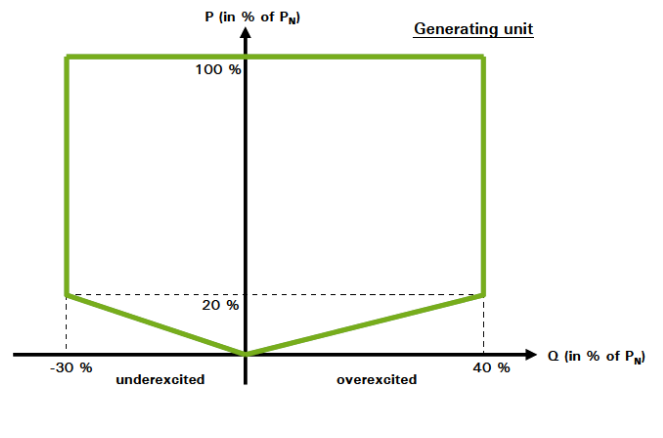
\includegraphics[width=0.8 \linewidth]{images_a7/gridcode.png}
        \caption{Requirement at the grid connection at the 33kV point}
        \label{fig:gridcode}   
\end{figure}
The Figure \ref{fig:gridcode} provided is the requirement to be followed by the offshore wind farm in order to achieve grid code compliance. The area within the "green line" is considered to be stable operation. The figure provides with limits within which a system should operate when it is under or overexcited. The operation of wind farm should be within these limits. The TSO specifies the code in order to maintain the system integrity and stable network operation. It also provides with requirements to maintain the grid under short disturbances.

\section*{Part C}
\begin{figure}[H]
    \centering
        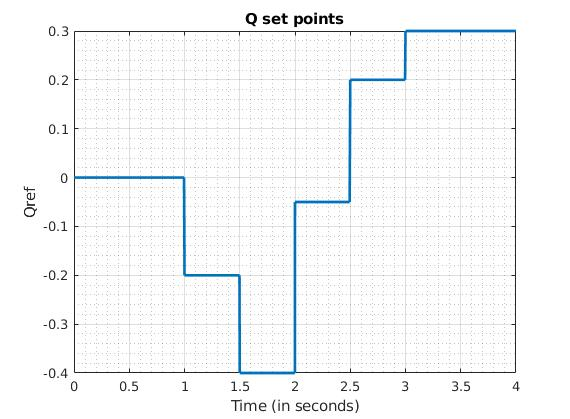
\includegraphics[width=0.8 \linewidth]{images_a7/Q_setpoints.jpg}
        \caption{Q set points}
        \label{fig:Q_set}   
\end{figure}

\begin{figure}[H]
    \centering
        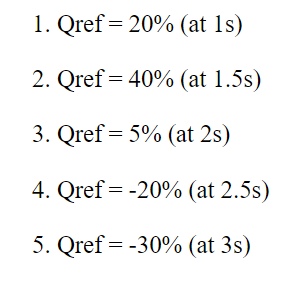
\includegraphics[width=0.2 \linewidth]{images_a7/Qref_setpoints.PNG}
        \caption{Q Ref}
        \label{fig:Q_ref}   
\end{figure}
The reactive power is set to a dynamic control , the controller gets a waveform as in \ref{fig:Q_set}, which is as per the requirement mentioned in \ref{fig:Q_ref}. Since the wind turbine is modelled as a static generator the values which are positive are taken as negative and vice versa.The step to the controller is passed through a first order transfer function so as to smooth the edges of the step.
From 0-1 s since the step is at zero, the reactive power also remains at zero.
From 1-1.5 s the system is in under excited mode and is still complying with the grid code.
From 1.5-2 s: The magnitude of under excited system is higher, but system is still grid complaint. 
From 2-2.5 s : The magnitude of the under excitation is again lowered,but the system is still  grid complaint.
From 2.5-3s : The system shifts from under excited to over excited mode, there is a zero crossing involved during this time step.This reversal of id can be visualized from \ref{fig:Idq}. This reversal still doesn't induce any harmonics because of the smooth waveform.
3s and above : As visualized from \ref{fig:Q_set} the value of set point is constant for a long period of time, this leads to a huge rise in the response by the controller as it is not able to find the stable point of operation. As visible from 
\ref{fig:PI} the controller output rises exponentially, this leads to a sudden spike in the reactive power that is supplied in the system, and the system fails to stay within the limits as per the grid compliance. This can clearly seen from the 
\ref{fig:Dynamic_control}, the value goes beyond the upper limit. 
If the system has to be grid complaint then the gain of the controller must be set accordingly (better tuning of the controller).

\begin{figure}[H]
    \centering
        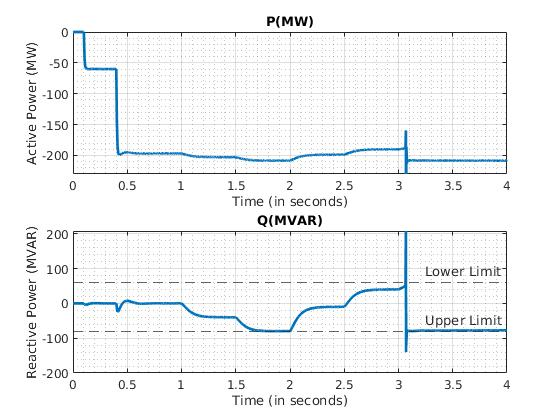
\includegraphics[width=0.5 \linewidth]{images_a7/dynamic_control.jpg}
        \caption{Dynamic Control of reactive power of the plant}
        \label{fig:Dynamic_control}   
\end{figure}
\begin{figure}[H]
    \centering
        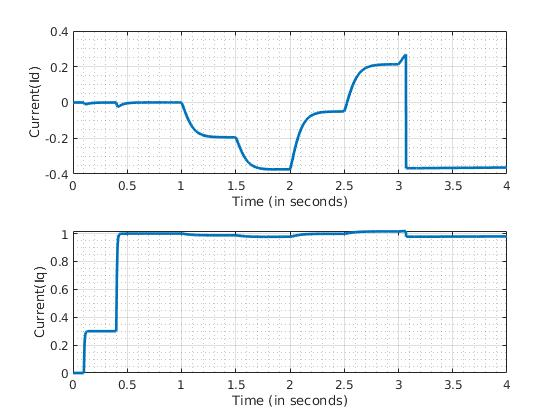
\includegraphics[width=0.5 \linewidth]{images_a7/Idq.jpg}
        \caption{Idq}
        \label{fig:Idq}   
\end{figure}
\begin{figure}[H]
    \centering
        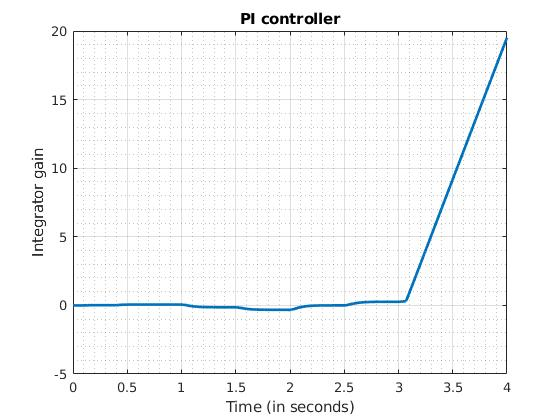
\includegraphics[width=0.5 \linewidth]{images_a7/PI.jpg}
        \caption{Integrator gain}
        \label{fig:PI}   
\end{figure}

\section*{Part D}
\begin{figure}[H]
    \centering
        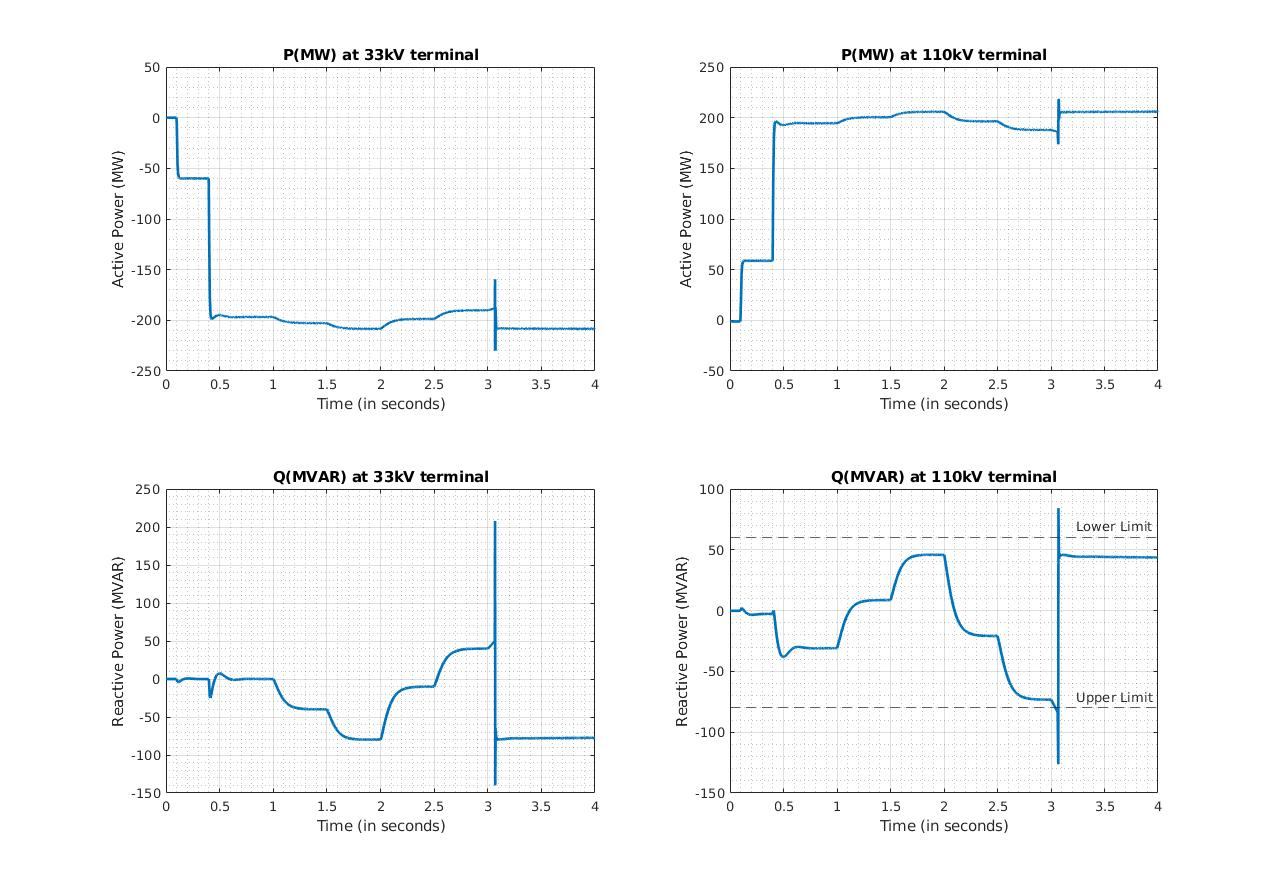
\includegraphics[width=0.8 \linewidth]{images_a7/20km_line.jpg}
        \caption{Active and Reactive Power at 33kV and 110kV terminals with a 20Km HVAC cable}
        \label{fig:20km_line}   
\end{figure}
Referring to Figures \ref{fig:20km_line} and \ref{fig:40km_line} for 110kV side, we see that when the length of the cable increases the reactive power increases due to higher capacitance in the line. The system is not able to satisfy grid code compliance. For a Transmission System Operator this means that there will be higher cost of expenditure due to increase in the length of the line and this might affect the system stability. 
\begin{figure}[H]
    \centering
        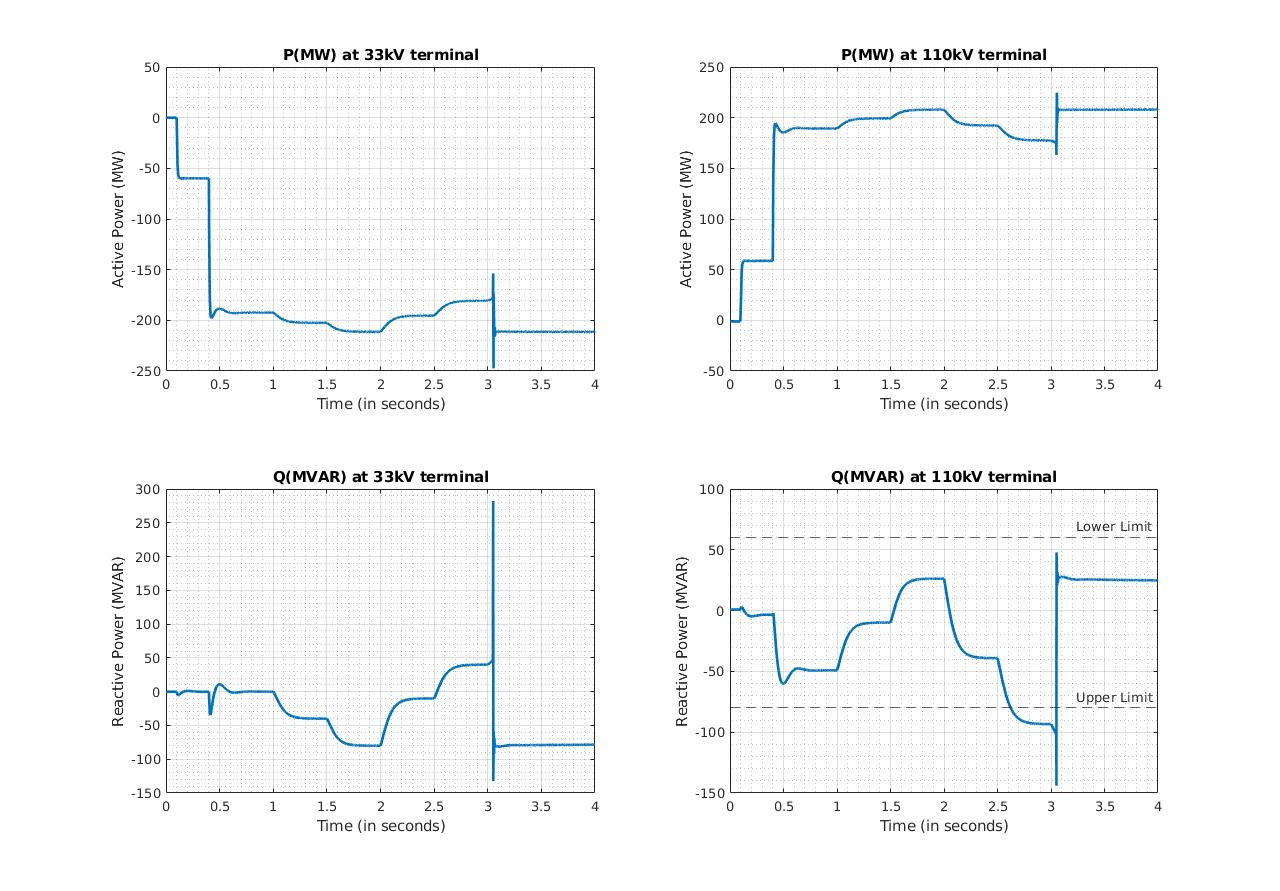
\includegraphics[width=0.8 \linewidth]{images_a7/40km_line.jpg}
        \caption{Active and Reactive Power at 33kV and 110kV terminals with a 40Km HVAC cable}
        \label{fig:40km_line}   
\end{figure}
\section*{Part E}
\begin{figure}[H]
    \centering
        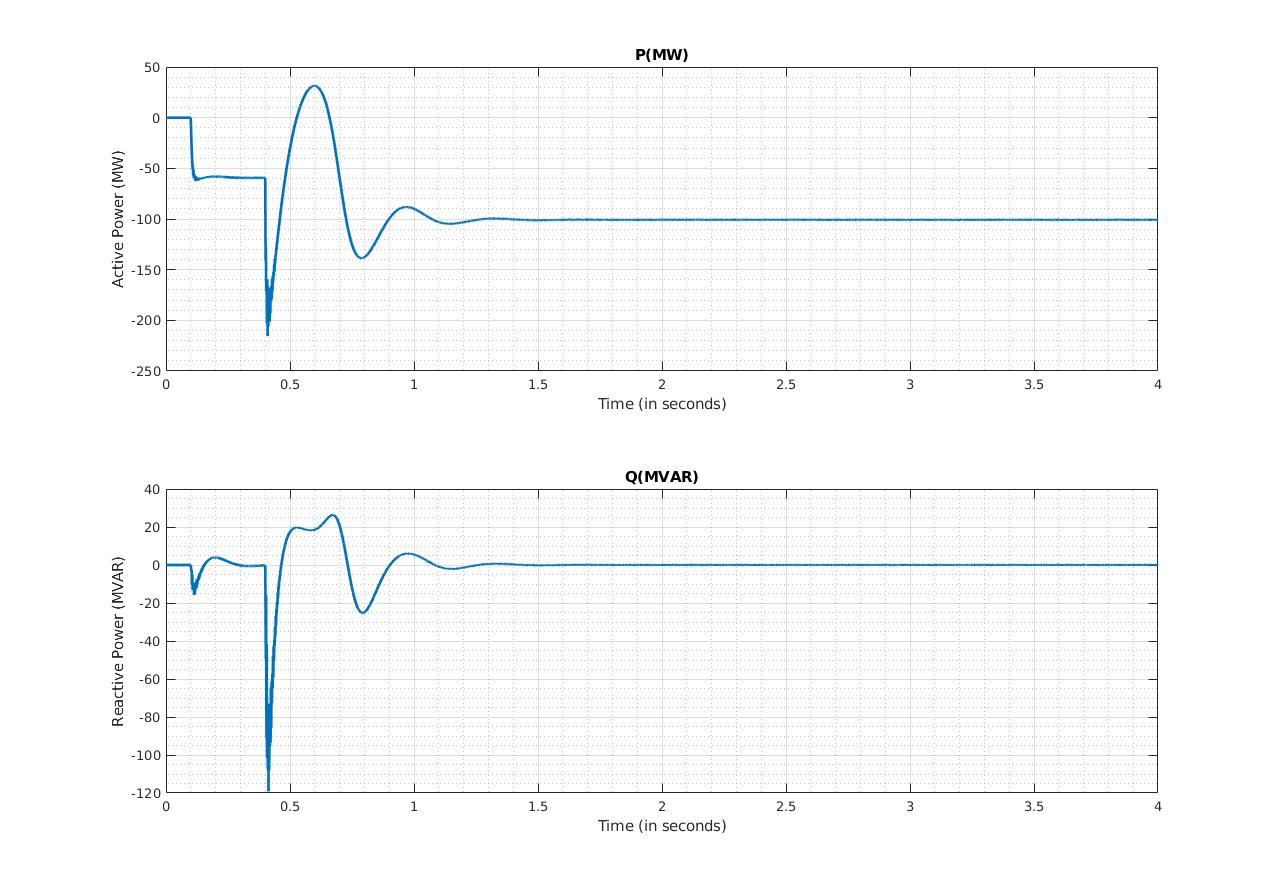
\includegraphics[width=0.6 \linewidth]{images_a7/criticalLength_160Km_stable.jpg}
        \caption{Critical Length of the cable for stable operation (160Km)}
        \label{fig:crit_160}   
\end{figure}
After changing the length of the cable in Load\_parameters.m script we observe that the critical length of the cable is 160Km (Figure \ref{fig:crit_160}). Beyond this length we observe (Figure \ref{fig:crit_170}) that there are oscillations introduced in the system. This can be attributed to the increase in the capacitance due to longer length of the cable and the reactive power is not enough compensate the higher capacitance.
\begin{figure}[H]
    \centering
        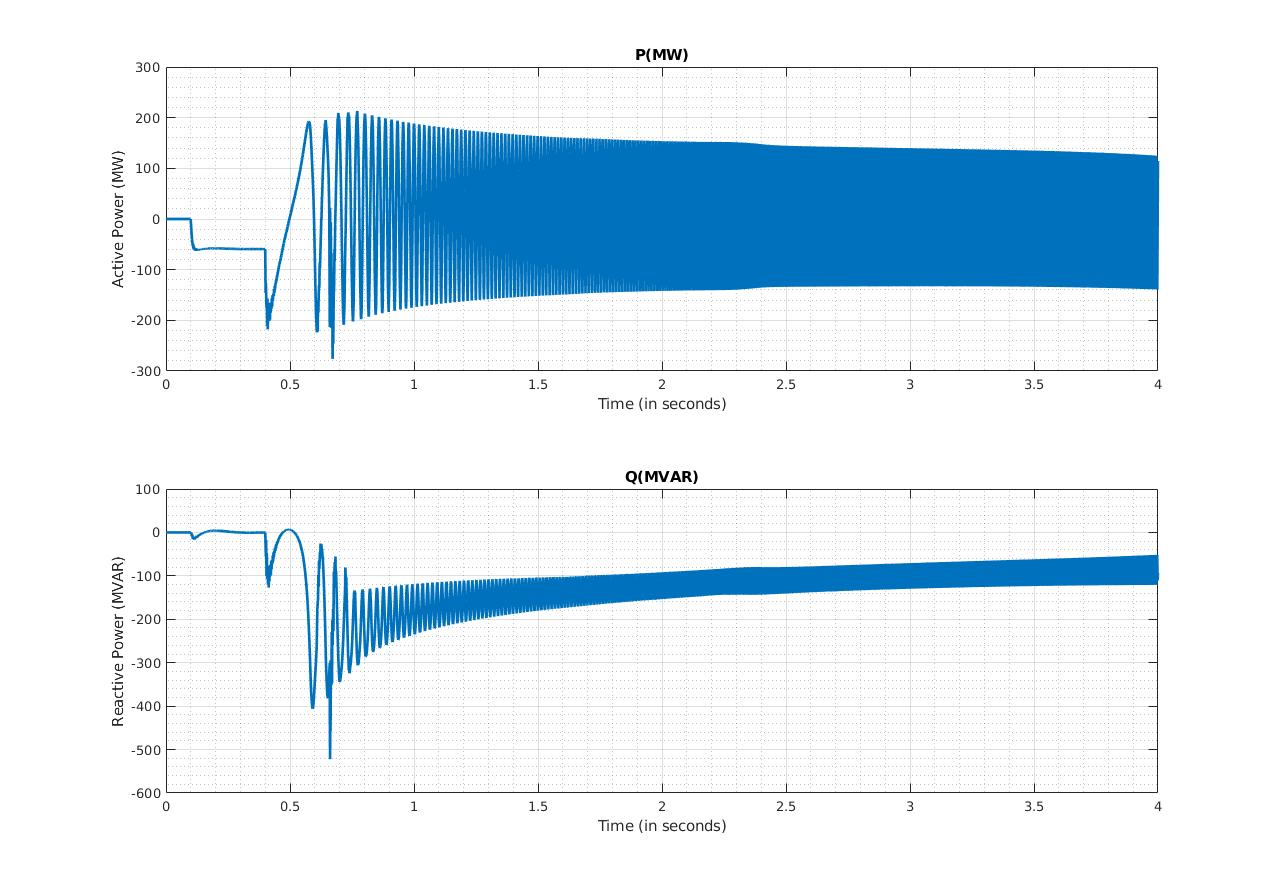
\includegraphics[width=0.6 \linewidth]{images_a7/criticalLength_170Km_unstable.jpg}
        \caption{Unstable Operation beyond 170Km}
        \label{fig:crit_170}   
\end{figure}
\section*{Part F}
Complying with grid code requirements and ensuring maximum energy output is done by installing a static synchronous compensator (STATCOM) at the point of common coupling (PCC). By applying a STATCOM system at the PCC, the plant owner or operator is able to automatically control the amount of reactive power, as well as address any voltage stability concerns.

A STATCOM will be able to quickly respond to grid events (with a response time of milliseconds), provides dynamic voltage control. Even on weak grids, the STATCOM device has the capability to control reactive power, limiting grid impedance, and ultimately enhancing the power output of a wind farm.